\documentclass[10pt]{beamer}
\usepackage{lmodern}
\usepackage{amsmath}
\usepackage{booktabs}
\usepackage{tabularx}
\usepackage{indent}
\usepackage{natbib}
\usepackage{tikz}
\usepackage{tikz-qtree}
\usetikzlibrary{positioning}
\usetheme{m}
\newcommand{\bs}{\ensuremath{\backslash}}
\newcommand{\deriv}[2]{%
\renewcommand{\arraystretch}{.5}
\begingroup
\footnotesize
    \begin{tabular}[t]{@{}*{#1}{c}}
        #2
    \end{tabular}
\endgroup
}
\newcommand{\ccgmc}[2]{\multicolumn{#1}{c}{#2}}
\newcommand{\w}[1]{\ccgmc{1}{#1}}
\newcommand{\uline}[1]{\ccgmc{#1}{\hrulefill}}
\newcommand{\frapply}[2]{\ccgmc{#1}{\ensuremath{\hrulefill_{R>}}}}
\newcommand{\fapply}[1]{\ccgmc{#1}{\ensuremath{\hrulefill_{>}}}}
\newcommand{\brapply}[1]{\ccgmc{#1}{\ensuremath{\hrulefill_{R<}}}}
\newcommand{\bapply}[1]{\ccgmc{#1}{\ensuremath{\hrulefill_{<}}}}
%\setbeamertemplate{caption}{\raggedright\insertcaption\par}
\newcolumntype{C}[1]{>{\hsize=#1\centering\arraybackslash}X}
\newcolumntype{R}[1]{>{\hsize=#1\raggedright\arraybackslash}X}
\addtobeamertemplate{frametitle}{}{\vspace*{-0.5cm}}
\title{\LARGE An Incremental Algorithm for Transition-based CCG Parsing}
\subtitle{\normalsize B. R. Ambati, T. Deoskar, M. Johnson and M. Steedman}
\author{Miyazawa Akira}
\institute{The Graduate University For Advanced Studies / National Institute of Informatics}
\begin{document}

\maketitle

\begin{frame}
    \frametitle{incrememtal parser}
    \nocite{ambati2015}
    What does ``Incremental'' mean?

    % See section 2.2
    \begin{indentation}{10pt}{0pt}
        An incremental parser
        computes the relationship between words as soon as
        it receives them from the input.
    \end{indentation}

    \bigskip

    Why is incrementality important?
    \begin{itemize}
        \item Statistical Machine Translation
        \item Automatic Speech Recognition
    \end{itemize}
\end{frame}

\begin{frame}
    \frametitle{baseline algorithm}
    Their baseline algorithm \texttt{NonInc} is based on \cite{zhang2011}.
    It has four actions.
    \begin{itemize}
        \item \textbf{Shift}

            Push a word from the input buffer to the stack and assign it with a CCG category.

        \item \textbf{Reduce Left}

            Pop the top two nodes from the stack, combine them into a new node and push it back onto the stack with a new category.
            The right node is the head and the left node is reduced.

        \item \textbf{Reduce Right}

            This is similar to the action above except that the left node is the head and the right node is reduced.

        \item \textbf{Unary}

            Change the category of the top node on the stack.
    \end{itemize}
\end{frame}

\begin{frame}
\frametitle{noninc algorithm}
\only<1>{\textbf{0}}
\only<2>{\textbf{1 Shift}}
\only<3>{\textbf{2 Shift}}
\only<4>{\textbf{3 Shift}}
\only<5>{\textbf{4 Shift}}
\only<6>{\textbf{5 Shift}}
\only<7>{\textbf{6 Reduce Right}}
\only<8>{\textbf{7 Reduce Right}}
\only<9>{\textbf{8 Reduce Right}}
\only<10>{\textbf{9 Shift}}
\only<11>{\textbf{10 Reduce Right}}
\only<12>{\textbf{11 Reduce Left}}
\only<13>{\textbf{Finish}}

Input buffer
\begin{center}
    {\onslide<1>{John\ \ }}
    {\onslide<1-2>{likes\ \ }}
    {\onslide<1-3>{mangoes\ \ }}
    {\onslide<1-4>{from\ \ }}
    {\onslide<1-5>{India\ \ }}
    {\onslide<1-9>{madly}}
\end{center}

Stack
\begin{center}
    {\only<2-11>{NP${}_\text{John}$\ \ }}
    {\only<3-8>{(S{\textbackslash}NP)/NP${}_\text{likes}$\ \ }}
    {\only<9-11>{S{\textbackslash}NP${}_\text{likes}$\ \ }}
    {\only<12->{S${}_\text{likes}$\ \ }}
    {\only<4-8>{NP${}_\text{mangoes}$\ \ }}
    {\only<5-6>{(NP\textbackslash{}NP)/NP${}_\text{from}$\ \ }}
    {\only<6>{NP${}_\text{India}$\ \ }}
    {\only<7>{NP\textbackslash{}NP${}_\text{from}$\ \ }}
    {\only<10>{(S\textbackslash{}NP)\textbackslash(S\textbackslash{}NP)${}_\text{madly}$\ \ }}
\end{center}

Dependency graph
\begin{center}
    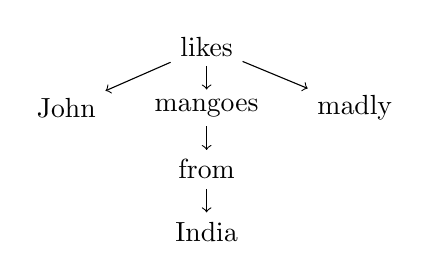
\begin{tikzpicture}
        \onslide<7->{\node (from) {from};}
        \onslide<7->{\node (india) [below= 0.3cm of from] {India};}
        \onslide<7->{\path[->] (from) edge (india);}
        \onslide<8->{\node (mangoes) [above= 0.3cm of from] {mangoes};}
        \onslide<8->{\path[->] (mangoes) edge (from);}
        \onslide<9->{\node (likes) [above= 0.3cm of mangoes] {likes};}
        \onslide<9->{\path[->] (likes) edge (mangoes);}
        \onslide<11->{\node (madly) [right= 0.5cm of mangoes] {madly};}
        \onslide<11->{\path[->] (likes) edge (madly);}
        \onslide<12->{\node (john) [left= 0.5cm of mangoes] {John};}
        \onslide<12->{\path[->] (likes) edge (john);}
    \end{tikzpicture}
\end{center}
\end{frame}

\begin{frame}
    \frametitle{problem in noninc}
    The algorithm above is not incremental.
    The dependncy graph starts to grow only after almost all the words are pushed to the stack.

    \bigskip

    To solve this problem, they introduce a \textbf{revealing} technique (\cite{pareschi1987}).
\end{frame}

\begin{frame}
\frametitle{revinc algorithm}
\only<1>{\textbf{0}}
\only<2>{\textbf{1 Shift}}
\only<3>{\textbf{2 Shift}}
\only<4>{\textbf{3-1 Type-Raising }}
\only<5>{\textbf{3-2 Reduce Left}}
\only<6>{\textbf{4 Shift}}
\only<7>{\textbf{5 Reduce Right}}
\only<8>{\textbf{6 Shift}}
\only<9>{\textbf{7 Shift}}
\only<10>{\textbf{8 Reduce Right}}
\only<11>{\textbf{\color{red}{9 Right Reveal}}}
\only<12>{\textbf{10 Shift}}
\only<13>{\textbf{\color{red}{11 Left Reveal}}}
\only<14>{\textbf{Finish}}

Input buffer
\begin{center}
    {\onslide<1>{John\ \ }}
    {\onslide<1-2>{likes\ \ }}
    {\onslide<1-5>{mangoes\ \ }}
    {\onslide<1-7>{from\ \ }}
    {\onslide<1-8>{India\ \ }}
    {\onslide<1-11>{madly}}
\end{center}

Stack
\begin{center}
    {\only<2-3>{NP${}_\text{John}$\ \ }}
    {\only<4>{S/(S{\textbackslash}NP)${}_\text{John}$\ \ }}
    {\only<3-4>{(S{\textbackslash}NP)/NP${}_\text{likes}$\ \ }}
    {\only<5-6>{S/NP${}_\text{likes}$\ \ }}
    {\only<7->{S${}_\text{likes}$\ \ }}
    {\only<6>{NP${}_\text{mangoes}$\ \ }}
    {\only<8-9>{(NP\textbackslash{}NP)/NP${}_\text{from}$\ \ }}
    {\only<10>{NP\textbackslash{}NP${}_\text{from}$\ \ }}
    {\only<9>{NP${}_\text{India}$\ \ }}
    {\only<12>{(S\textbackslash{}NP)\textbackslash(S\textbackslash{}NP)${}_\text{madly}$}}
\end{center}

Dependency graph
\begin{columns}
    \begin{column}{0.3\textwidth}
    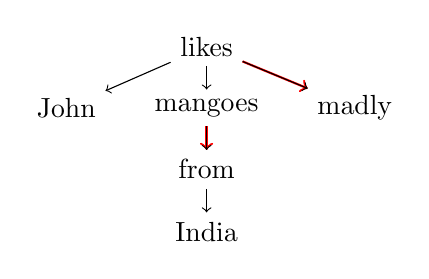
\begin{tikzpicture}
        \onslide<10->{\node (from) {from};}
        \onslide<10->{\node (india) [below= 0.3cm of from] {India};}
        \onslide<10->{\path[->] (from) edge (india);}
        \onslide<7->{\node (mangoes) [above= 0.3cm of from] {mangoes};}
        \onslide<11>{\path[->,red,thick] (mangoes) edge (from);}
        \onslide<12->{\path[->] (mangoes) edge (from);}
        \onslide<5->{\node (likes) [above= 0.3cm of mangoes] {likes};}
        \onslide<7->{\path[->] (likes) edge (mangoes);}
        \onslide<13->{\node (madly) [right= 0.5cm of mangoes] {madly};}
        \onslide<13>{\path[->,red,thick] (likes) edge (madly);}
        \onslide<14>{\path[->] (likes) edge (madly);}
        \onslide<5->{\node (john) [left= 0.5cm of mangoes] {John};}
        \onslide<5->{\path[->] (likes) edge (john);}
    \end{tikzpicture}
    \end{column}
    \begin{column}{0.4\textwidth}
        \only<11>{%
            \deriv{3}{%
                \ccgmc{2}{S${}_\text{likes}$}                                           & \w{NP{\textbackslash}NP${}_\text{from}$}  \\
                \frapply{2}                                                             & \\
                \w{S/NP${}_\text{likes}$}               & \w{NP${}_\text{mangoes}$}     & \\
                                                        & \bapply{2}                      \\
                                                        & \ccgmc{2}{NP}                   \\
                \fapply{3}                                                                \\
                \ccgmc{3}{S}                                                              \\
            }
        }
        \only<13>{%
            \deriv{3}{%
                \ccgmc{2}{S${}_\text{likes}$}                                                        & \w{(S{\textbackslash}NP)\textbackslash(S{\textbackslash}NP)${}_\text{madly}$}  \\
                \brapply{2}                                                                          &                                                                                \\
                \w{NP${}_\text{John}$}                & \w{S{\textbackslash}NP${}_\text{likes}$}     &                                                                                \\
                                                      & \bapply{2}                                                                                                                    \\
                                                      & \ccgmc{2}{S{\textbackslash}NP}                                                                                                \\
                \bapply{3}                                                                                                                                                            \\
                \ccgmc{3}{S}                                                                                                                                                          \\
            }
        }
    \end{column}
\end{columns}
\end{frame}

\begin{frame}
    \frametitle{revealing actions}
    \begin{enumerate}
        \item \textbf{Left Reveal} (\texttt{LRev})

            Pop the top two nodes in the stack (left, right).
            Identify the left node's child with a subject dependency.
            Abstract over this child node and split the category of
            left node into two categories.
            Combine the nodes using CCG combinators accodingly.

            \bigskip

            \begin{center}
                \begin{tabular}[h]{@{}*{3}{c}}
                \ccgmc{2}{S${}_\text{likes}$}                                                        & \w{(S{\textbackslash}NP)\textbackslash(S{\textbackslash}NP)${}_\text{madly}$}  \\
                \brapply{2}                                                                          &                                                                                \\
                \w{NP${}_\text{John}$}                & \w{S{\textbackslash}NP${}_\text{likes}$}     &                                                                                \\
                                                      & \bapply{2}                                                                                                                    \\
                                                      & \ccgmc{2}{S{\textbackslash}NP}                                                                                                \\
                \bapply{3}                                                                                                                                                            \\
                \ccgmc{3}{S}                                                                                                                                                          \\
                \end{tabular}
            \end{center}
    \end{enumerate}
\end{frame}

\begin{frame}
    \frametitle{revealing actions}
    \begin{enumerate}
        \setcounter{enumi}{1}
        \item \textbf{Right Reveal} (\texttt{RRev})

            Pop the top two nodes in the stack (left, right).
            Check the right periphery of the left node in the dependency graph,
            extract all the nodes with compatible CCG categories and identify all the possible nodes that the right node can combine with.
            Abstract over this node, split the category into two categories accordingly and combine the nodes using CCG combinators.

            \bigskip

            \begin{center}
                \begin{tabular}[h]{@{}*{3}{c}}
                \ccgmc{2}{S${}_\text{likes}$}                                           & \w{NP{\textbackslash}NP${}_\text{from}$}  \\
                \frapply{2}                                                             & \\
                \w{S/NP${}_\text{likes}$}               & \w{NP${}_\text{mangoes}$}     & \\
                                                        & \bapply{2}                      \\
                                                        & \ccgmc{2}{NP}                   \\
                \fapply{3}                                                                \\
                \ccgmc{3}{S}                                                              \\
                \end{tabular}
            \end{center}
    \end{enumerate}
\end{frame}

\begin{frame}
    % https://catalog.ldc.upenn.edu/desc/addenda/LDC2005T13.html
    \frametitle{data and settings}
        Data: CCGbank
        \begin{itemize}
            \item training: sections 02--21
            \item development: section 00
            \item testing: section 23
        \end{itemize}

        POS tagger:
        \begin{indentation}{10pt}{0pt}
            C\&C POS tagger
        \end{indentation}

        Supertagger:
        \begin{indentation}{10pt}{0pt}
            C\&C supertagger
        \end{indentation}
\end{frame}

\begin{frame}
    \frametitle{features}
    \begingroup
    \scriptsize
    \begin{itemize}
        \item NonInc

            Features based on the top four nodes in the stack and the next four words in the input buffer.

            \begin{center}
                \begin{table}
                        \begin{tabularx}{0.95\textwidth}{C{10pt}R{250pt}}
                        \toprule
                        \multicolumn{2}{c}{feature templates} \\
                        \toprule
                        1 & S${}_0$wp, S${}_{0}$c, S${}_0$pc, S${}_0$wc,
                        S${}_1$wp, S${}_1$c, S${}_1$pc, S${}_1$wc,
                        S${}_2$pc, S${}_2$wc,
                        S${}_{3}$pc, S${}_3$wc, \\
                        \midrule
                        2 & Q${}_0$wp, Q${}_1$wp, Q${}_2$wp, Q${}_3$wp, \\
                        \midrule
                        3 & S${}_0$Lpc, S${}_0$Lwc, S${}_0$Rpc, S${}_0$Rwc,
                        S${}_0$Upc, S${}_0$Uwc,
                        S${}_1$Lpc, S${}_1$Lwc, S${}_1$Rpc, S${}_1$Rwc,
                        S${}_1$Upc, S${}_1$Uwc, \\
                        \midrule
                        4 & S${}_0$wcS${}_1$wc,
                        S${}_0$cS${}_1$w,
                        S${}_0$wS${}_1$c,
                        S${}_0$cS${}_1$c,
                        S${}_0$wcQ${}_0$wp,
                        S${}_0$cQ${}_0$wp,
                        S${}_0$wcQ${}_0$p,
                        S${}_0$cQ${}_0$p,
                        S${}_1$wcQ${}_0$wp,
                        S${}_1$cQ${}_0$wp,
                        S${}_1$wcQ${}_0$p,
                        S${}_1$cQ${}_0$p, \\
                        \midrule
                        5 & S${}_0$wcS${}_1$cQ${}_0$p,
                        S${}_0$cS${}_1$wcQ${}_0$p,
                        S${}_0$cS${}_1$cQ${}_0$wp,
                        S${}_0$cS${}_1$cQ${}_0$p,
                        S${}_0$pS${}_1$pQ${}_0$p,
                        S${}_0$wcQ${}_0$pQ${}_1$p,
                        S${}_0$cQ${}_0$wpQ${}_1$p,
                        S${}_0$cQ${}_0$pQ${}_1$wp,
                        S${}_0$cQ${}_0$pQ${}_1$p,
                        S${}_0$pQ${}_0$pQ${}_1$p,
                        S${}_0$wcS${}_1$cS${}_2$c,
                        S${}_0$cS${}_1$wcS${}_2$c,
                        S${}_0$cS${}_1$cS${}_2$wc,
                        S${}_0$cS${}_1$cS${}_2$,
                        S${}_0$pS${}_1$pS${}_2$, \\
                        \midrule
                        6 & S${}_0$cS${}_0$HcS${}_0$Lc,
                        S${}_0$cS${}_0$HcS${}_0$Rc,
                        S${}_1$cS${}_1$HcS${}_1$Rc,
                        S${}_0$cS${}_0$RcQ${}_0$p,
                        S${}_0$cS${}_0$RcQ${}_0$w,
                        S${}_0$cS${}_0$LcS${}_1$c,
                        S${}_0$cS${}_0$LcS${}_1$w,
                        S${}_0$cS${}_1$cS${}_1$Rc,
                        S${}_0$wS${}_1$cS${}_1$Rc, \\
                        \bottomrule
                    \end{tabularx}
                \end{table}
            \end{center}

            \bigskip

        \item RevInc

            $\uparrow$ + B${}_1$c and B${}_1$cS${}_0$c, where B${}_1$ is the bottom most node in the right periphery.
    \end{itemize}
    \endgroup
\end{frame}

\begin{frame}
    \frametitle{Measures of incrementality}
    Measures of incrementality:
    \begin{itemize}
        \item \textbf{Connectedness}

            the average number of nodes in the stack before shifting

        \item \textbf{Waiting time}

            the number of nodes that need to be shifted to the stack
            before a dependency between any two nodes in the stack is resolved
    \end{itemize}

    \smallskip

    \begin{center}
        \begin{table}
        \caption{Connectedness and waiting time.}
        \begin{tabular}{ccc}
            \toprule
            Algorithm  & Connectedness & Waiting Time  \\
            \midrule
            NonInc     & 4.62          & 2.98          \\
            RevInc     & \textbf{2.15} & \textbf{0.69} \\
            \bottomrule
        \end{tabular}
        \end{table}
    \end{center}
\end{frame}

\begin{frame}
    \frametitle{results and analysis}
    \begingroup
    \scriptsize
    \begin{center}
    \begin{table}
    \caption{Performance on the development data\footnote{`U' stands for unlabaled and `L' stands for labeles. `P', `R' and `F' are precision, recall and F-score respectively.}.}
        \begin{table}[h]
            \begin{tabular}{cccccccc}
                \toprule
                Algorithm        & UP
                                                  & UR             & UF             & LP             & LR             & LF             & Cat Acc. \\
                \midrule
                NonInc (beam=1)  & \textbf{92.57} & 82.60          & 87.30          & \textbf{85.12} & 75.96          & 80.28          & 91.10 \\
                RevInc (beam=1)  & 91.62          & \textbf{85.94} & \textbf{88.69} & 83.42          & \textbf{78.25} & \textbf{80.75} & 90.87 \\
                \midrule
                NonInc (beam=16) & 92.71          & 89.66          & 91.16          & 85.78          & 82.96          & 84.35          & 92.51 \\
                Z\&C (beam=16)   & -              & -              & -              & 87.15          & 82.95          & 85.00          & 92.77 \\
                \bottomrule
            \end{tabular}
        \end{table}
    \end{table}
    \end{center}
    \endgroup
    \smallskip

    \begin{itemize}
        \item NonInc gets higher precision because it can use more context while making a decision.
        \item RevInc achieves higher recall because information on nodes is available even after they are reduced.
    \end{itemize}
\end{frame}

\begin{frame}
    \frametitle{results and analysis}
    \begingroup
    \small
    \begin{center}
    \begin{table}
        \caption{Label-wise F-score of RevInc and NonInc parsers.}
            \begin{tabular}{ccc}
            \toprule
            Category                                                               & RevInc         & NonInc         \\
            \midrule
            (NP{\textbackslash}NP)/\textbf{NP}                                     & 81.36          & \textbf{83.21} \\
            (NP\textbackslash\textbf{NP})/NP                                       & 78.66          & \textbf{82.94} \\
            ((S{\textbackslash}NP)\textbackslash(S{\textbackslash}NP))/\textbf{NP} & 65.09          & \textbf{66.98} \\
            ((S{\textbackslash}NP)\textbackslash\textbf{(S{\textbackslash}NP)})/NP & 62.69          & \textbf{65.89} \\
            (S[dcl]{\textbackslash}NP)/\textbf{NP}                                 & \textbf{78.96} & 78.29          \\
            (S[dcl]\textbackslash\textbf{NP})/NP                                   & \textbf{76.71} & 75.22          \\
            (S{\textbackslash}NP)\textbackslash\textbf{(S{\textbackslash}NP)}      & \textbf{80.49} & 76.90          \\
            \bottomrule
            \end{tabular}
    \end{table}
    \end{center}
    \endgroup

    \smallskip

    \begin{itemize}
        \item NonInc performs better in labels corresponding to PP due to the availability of more context.
        \item RevInc has advantage in the case of verbal arguments and verbal modifiers as the effect of ``reveal'' actions.
    \end{itemize}
\end{frame}

\begin{frame}
    \frametitle{parsing speed}
    Parsing speed:
    \begin{itemize}
        \item NonInc parses 110 sentences/sec.
        \item RevInc parses 125 sentences/sec.
    \end{itemize}

    \bigskip

    Significant amount of parsing time is spent on the feature extraction step.
    But in RevInc, usually only two nodes have their feature extracted because connectedness = 2.15,
    while all four nodes have to be processed in NonInc (connectedness = 4.62).

    \smallskip

    Complex actions, \texttt{LRev} and \texttt{RRev} are rarely used (5\%).
\end{frame}

\begin{frame}
    \frametitle{results and analysis}
    \begingroup
    \scriptsize
    \begin{center}
    \begin{table}
        \caption{Performance on the test data.}
        \begin{tabular}{cccccccc}
            \toprule
            Algorithm        & UP             & UR             & UF             & LP             & LR             & LF             & Cat Acc. \\
            \midrule
            NonInc (beam=1)  & \textbf{92.45} & 82.16          & 87.00          & \textbf{85.59} & 76.06          & 80.55          & 91.39 \\
            RevInc (beam=1)  & 91.83          & \textbf{86.35} & \textbf{89.00} & 84.02          & \textbf{79.00} & \textbf{81.43} & 91.17 \\
            \midrule
            NonInc (beam=16) & 92.68          & 89.57          & 91.10          & 86.20          & 83.32          & 84.74          & 92.70 \\
            Z\&C (beam=16)   & -              & -              & -              & 87.43          & 83.61          & 85.48          & 93.12 \\
            Hassan et al. 09 & -              & -              & 86.31          & -              & -              & -              & -     \\
            \bottomrule
        \end{tabular}
    \end{table}
    \end{center}
    \endgroup

     F-scores are improved compared to NonInc in both unlabaled and labeled cases.
\end{frame}

\begin{frame}
    \frametitle{future plan}
    \begin{itemize}
        \item Use information about lexical category probabilities (\cite{auli2011}).

        \item Explore the limited use of a beam to handle lexical ambiguity.
        \item Use a dynamic oracle strategy (\cite{xu2014}).
        \item Apply the method to SMT and ASR.
    \end{itemize}
\end{frame}

\begin{frame}
    \frametitle{conclusion}
    \begin{itemize}
        \item They designed and implemented an incremental CCG parser by introducing a technique called revealing.
        \item The parser got high scores in two measures of incrementality: connectedness and waiting time.
        \item It performs better in parsing in the view of recall and F-score. (labeled: +0.88\%, unlabeld: +2.0\%)
        \item It parses sentences faster.
    \end{itemize}
\end{frame}

\begin{frame}
  \frametitle{References}

  \bibliographystyle{apalike}
  \bibliography{incremental_ccg}

\end{frame}
\end{document}
